\chapter{Scomposizione del VAB}
\section{Considerazioni iniziali}
Per il calcolo delle equazioni dinamiche del sistema siamo andati a considerare ogni singolo corpo rigido componente il sistema, calcolandone le grandezze fisiche di posizione e velocità, seguendo un approccio cartesiano. 
Nello specifico abbiamo considerato il sistema composto da:
\begin{itemize}
	\item Asta
	\item Utente a bordo dello chassis
	\item Chassis (nel corso della trattazione sarà chiamata talvolta anche base)
	\item Ruota (che poi sarà considerata con un contributo doppio, essendo il VAB composto da due ruote)
\end{itemize}

Ognuno di questi corpi rigidi separati è individuato da un punto, che ne rappresenta il centro di massa (o baricentro del corpo stesso): avremo quindi questo insieme di punti caratterizzanti il sistema (figura ~\ref{fig:VAB_baricentri})

\begin{itemize}
	\item \textbf{$P_a$}
	\item \textbf{$P_b$}
	\item \textbf{$P_c$}
	\item \textbf{$P_r$}
\end{itemize}

\begin{figure}[H]
	\centering   	
	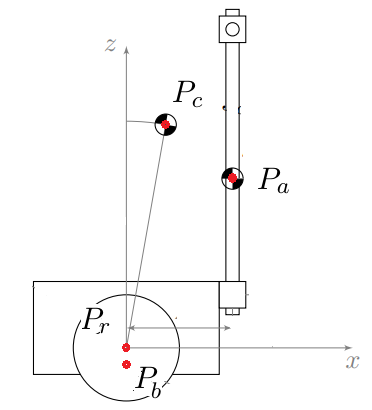
\includegraphics[width=0.4\textwidth]{Immagini/VAB_baricentrum.png}
	\caption{Baricentri dei singoli corpi rigidi}
	\label{fig:VAB_baricentri}
\end{figure} 

\section{Grandezze di supporto}
Prima di andare a definire le componenti di energia potenziale e cinetica di ogni singolo corpo, siamo andati ad introdurre alcune grandezze geometriche di supporto che definiremo qui di seguito.

Nello specifico abbiamo introdotto i seguenti parametri, specificati anche in figura ~\ref{fig:VAB_lunghezze}:
\begin{itemize}
	\item \textbf{$l_a$}: rappresenta la congiungente tra il centro del sistema di riferimento e il centro dell'asta, utilizzata appunto come manubrio, che abbiamo individuato come
	\begin{center}
		{\Large $\sqrt{(\frac{h_a}{2} + \frac{h_b}{2})^2 + (\frac{w_b}{2})^2}$}
	\end{center}
	\item \textbf{$l_c$}: (TODO: check) questa grandezza invece rappresenta per noi l'altezza del baricentro del corpo dell'utente, la quale ovviamente andrà a dipendere dal valore di inclinazione del corpo stesso.
	Considerando il corpo inzialmente in posizione verticale, avremo che questa grandezza corrisponde alla congiungente dal centro del sistema di riferimento al punto $P_c$, che equivale a dire che
	\begin{center}
		$l_c = 0.55\bullet h_c + \frac{h_b}{2}$
	\end{center}
	\item \textbf{$l_b$}: spostamento verso il basso, lungo l'asse z, del baricentro dello chassis. Da specifiche del progetto sappiamo che questa grandezza ha valore (con segno negativo) di:
	\begin{center}
		$l_b = 0.1 m$
	\end{center}
	\item \textbf{$\beta$}: angolo formato con la verticale dalla congiungente tra il centro del sistema di riferimento e il punto $P_a$. Si ricava, con un semplice approccio trigonometrico, che l'angolo in questione ha questa forma
	\begin{center}
		$\arctan{(\frac{\frac{w_b}{2}}{\frac{h_a}{2} + \frac{h_b}{2}})}$
	\end{center}
\end{itemize}

\begin{figure}[h]
	\centering   	
	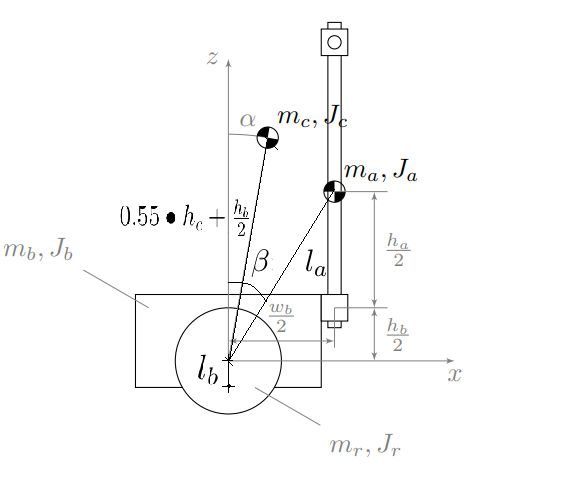
\includegraphics[width=0.6\textwidth]{Immagini/VAB_additionalMeasures.png}
	\caption{Lunghezze di supporto}
	\label{fig:VAB_lunghezze}
\end{figure}

\section{Calcolo componenti dinamiche e potenziali per ogni corpo rigido del sistema}
Per ognuno dei corpi rigidi definiti in precedenza siamo andati appunto a calcolare:

\begin{itemize}
	\item \textbf{Coordinate spaziali P} espresse nel sistema di riferimento XZ. A queste due coordinate cartesiane ne va aggiunta una terza, relativa alle coordinate angolari (per poter tener così conto dei contirbuti inerziali);
	\item \textbf{Vettore delle velocità V} $\rightarrow$ vettore $3\times 1$
	\item \textbf{Matrice delle masse M} $\rightarrow$ matrice $3\times 3$
	\item \textbf{Energia cinetica T} $\rightarrow \frac{1}{2}\bullet V^T \bullet M \bullet V$
	\item \textbf{Energia potenziale U}
	\item \textbf{Lagrangiana \textit{parziale} L}
\end{itemize}

\subsection{Asta}
\begin{itemize}
	\item \textbf{$P_a = \left(\begin{array}{c}
		r\,\phi \left(t\right)+l_a \,\mathrm{sin}\left(\beta +\theta \left(t\right)\right)\\
		l_a \,\mathrm{cos}\left(\beta +\theta \left(t\right)\right)\\
		\theta \left(t\right)
		\end{array}\right)$}

	\item \textbf{$V_a = \left(\begin{array}{c}
		r\,\dot{\phi \left(t\right)}+l_a \,\mathrm{cos}\left(\beta +\theta \left(t\right)\right)\,\dot{\theta \left(t\right)}\\
		-l_a \,\mathrm{sin}\left(\beta +\theta \left(t\right)\right)\,\dot{\theta \left(t\right)}\\
		\dot{\theta \left(t\right)}
		\end{array}\right)$}
	
	\item \textbf{$M_a = \left(\begin{array}{ccc}
		m_a  & 0 & 0\\
		0 & m_a  & 0\\
		0 & 0 & m_a \,{l_a }^2 +J_a 
		\end{array}\right)$}
	
	\item \textbf{$T_a = m_a \,{l_a }^2 \,{{\left(\dot{\theta \left(t\right)}\right)}}^2 +\frac{m_a \,r^2 \,{{\left(\dot{\phi \left(t\right)}\right)}}^2 }{2}+\frac{J_a \,{{\left(\dot{\theta \left(t\right)}\right)}}^2 }{2}+m_a \,\mathrm{cos}\left(\beta +\theta \left(t\right)\right)\,l_a \,r\,\dot{\theta \left(t\right)}\,\dot{\phi \left(t\right)}$}
	
	\item \textbf{$U_a = g\,l_a \,m_a \,\mathrm{cos}\left(\beta +\theta \left(t\right)\right)$}
	
	\item \textbf{$L_a = m_a \,{l_a }^2 \,{{\left(\dot{\theta \left(t\right)}\right)}}^2 +\frac{m_a \,r^2 \,{{\left(\dot{\phi \left(t\right)}\right)}}^2 }{2}+\frac{J_a \,{{\left(\dot{\theta \left(t\right)}\right)}}^2 }{2}+m_a \,\mathrm{cos}\left(\beta +\theta \left(t\right)\right)\,l_a \,r\,\dot{\theta \left(t\right)}\,\dot{\phi \left(t\right)}-g\,m_a \,\mathrm{cos}\left(\beta +\theta \left(t\right)\right)\,l_a$}
\end{itemize}
\subsection{Chassis (base)}
\begin{itemize}
	\item \textbf{$P_b = \left(\begin{array}{c}
		r\,\phi \left(t\right)-l_b \,\mathrm{sin}\left(\theta \left(t\right)\right)\\
		-l_b \,\mathrm{cos}\left(\theta \left(t\right)\right)\\
		\theta \left(t\right)
		\end{array}\right)$}
	
	\item \textbf{$V_b = \left(\begin{array}{c}
		r\,\dot{\phi \left(t\right)}-l_b \,\mathrm{cos}\left(\theta \left(t\right)\right)\,\dot{\theta \left(t\right)}\\
		l_b \,\mathrm{sin}\left(\theta \left(t\right)\right)\,\dot{\theta \left(t\right)}\\
		\dot{\theta \left(t\right)}
		\end{array}\right)$}
	
	\item \textbf{$M_b = \left(\begin{array}{ccc}
		m_b  & 0 & 0\\
		0 & m_b  & 0\\
		0 & 0 & m_b \,{l_b }^2 +J_b 
		\end{array}\right)$}
	
	\item \textbf{$T_b = m_b \,{l_b }^2 \,{{\left(\dot{\theta \left(t\right)}\right)}}^2 +\frac{m_b \,r^2 \,{{\left(\dot{\phi \left(t\right)}\right)}}^2 }{2}+\frac{J_b \,{{\left(\dot{\theta \left(t\right)}\right)}}^2 }{2}-m_b \,\mathrm{cos}\left(\theta \left(t\right)\right)\,l_b \,r\,\dot{\theta \left(t\right)}\,\dot{\phi \left(t\right)}$}
	
	\item \textbf{$U_b = -g\,l_b \,m_b \,\mathrm{cos}\left(\theta \left(t\right)\right)$}
	
	\item \textbf{$L_b = m_b \,{l_b }^2 \,{{\left(\dot{\theta \left(t\right)}\right)}}^2 +\frac{m_b \,r^2 \,{{\left(\dot{\phi \left(t\right)}\right)}}^2 }{2}+\frac{J_b \,{{\left(\dot{\theta \left(t\right)}\right)}}^2 }{2}-m_b \,\mathrm{cos}\left(\theta \left(t\right)\right)\,l_b \,r\,\dot{\theta \left(t\right)}\,\dot{\phi \left(t\right)}+g\,m_b \,\mathrm{cos}\left(\theta \left(t\right)\right)\,l_b$}
\end{itemize}
\subsection{Utente}
\begin{itemize}
	\item \textbf{$P_c = \left(\begin{array}{c}
		r\,\phi \left(t\right)+l_c \,\mathrm{sin}\left(\alpha +\theta \left(t\right)\right)\\
		l_c \,\mathrm{cos}\left(\alpha +\theta \left(t\right)\right)\\
		\alpha +\theta \left(t\right)
		\end{array}\right)$}
	
	\item \textbf{$V_c = \left(\begin{array}{c}
		r\,\dot{\phi \left(t\right)}+l_c \,\mathrm{cos}\left(\alpha +\theta \left(t\right)\right)\,\dot{\theta \left(t\right)}\\
		-l_c \,\mathrm{sin}\left(\alpha +\theta \left(t\right)\right)\,\dot{\theta \left(t\right)}\\
		\dot{\theta \left(t\right)}
		\end{array}\right)$}
	
	\item \textbf{$M_c = \left(\begin{array}{ccc}
		m_c  & 0 & 0\\
		0 & m_c  & 0\\
		0 & 0 & m_c \,{l_c }^2 +J_c 
		\end{array}\right)$}
	
	\item \textbf{$T_c = m_c \,{l_c }^2 \,{{\left(\dot{\theta \left(t\right)}\right)}}^2 +\frac{m_c \,r^2 \,{{\left(\dot{\phi \left(t\right)}\right)}}^2 }{2}+\frac{J_c \,{{\left(\dot{\theta \left(t\right)}\right)}}^2 }{2}+m_c \,\mathrm{cos}\left(\alpha +\theta \left(t\right)\right)\,l_c \,r\,\dot{\theta \left(t\right)}\,\dot{\phi \left(t\right)}$}
	
	\item \textbf{$U_c = g\,l_c \,m_c \,\mathrm{cos}\left(\alpha +\theta \left(t\right)\right)$}
	
	\item \textbf{$L_c = m_c \,{l_c }^2 \,{{\left(\dot{\theta \left(t\right)}\right)}}^2 +\frac{m_c \,r^2 \,{{\left(\dot{\phi \left(t\right)}\right)}}^2 }{2}+\frac{J_c \,{{\left(\dot{\theta \left(t\right)}\right)}}^2 }{2}+m_c \,\mathrm{cos}\left(\alpha +\theta \left(t\right)\right)\,l_c \,r\,\dot{\theta \left(t\right)}\,\dot{\phi \left(t\right)}-g\,m_c \,\mathrm{cos}\left(\alpha +\theta \left(t\right)\right)\,l_c$}
\end{itemize}
\subsection{Ruota}
\begin{itemize}
	\item \textbf{$P_r = \left(\begin{array}{c}
		r\,\phi \left(t\right)\\
		0\\
		\phi \left(t\right)
		\end{array}\right)$}
	
	\item \textbf{$V_r = \left(\begin{array}{c}
		r\,\dot{\phi \left(t\right)}\\
		0\\
		\dot{\phi \left(t\right)}
		\end{array}\right)$}
	
	\item \textbf{$M_r = \left(\begin{array}{ccc}
		m_r  & 0 & 0\\
		0 & m_r  & 0\\
		0 & 0 & J_r 
		\end{array}\right)$} \label{matrix:mr}
	
	\item \textbf{$T_r = \frac{{\left(m_r \,r^2 +J_r \right)}\,{{\left(\dot{\phi \left(t\right)}\right)}}^2 }{2}$}
	
	\item \textbf{$U_r = 0$}
	
	\item \textbf{$L_r = \frac{{\left(m_r \,r^2 +J_r \right)}\,{{\left(\dot{\phi \left(t\right)}\right)}}^2 }{2}$}
\end{itemize}

\subsection{Veicolo completo}
Una volta trovati le componenti dinamiche dei singoli corpi rigidi, possiamo andare a definire l'energia cinetica e potenziale totale del sistema, per poter poi andare a calcolare l'equazione di Lagrange per l'intero sistema.
In sostanza quindi avremo:
\begin{center}
	$L = L_a + L_b + L_c + 2 \bullet L_r$
\end{center}

\subsection{Note sul calcolo delle componenti dinamiche}
\begin{itemize}
	\item Nel calcolo della matrice di massa abbiamo considerato tre componenti:
	\begin{itemize}
		\item Componente di massa lungo x;
		\item Componente di massa lungo z;
		\item Componente di massa rotazionale: dalla meccanica è noto che, un corpo con una certa massa che si trova in uno stato di rotazione, avrà un contirbuto inerziale che dipende dal braccio rispetto al quale avviene la rotazione.
		Nello specifico, per ogni singolo corpo rigido che è stato preso in esame, abbiamo considerato, secondo il teorema di \textit{Huygens-Steiner}, il quale permette di definire l'inerzia di un corpo come la somma di due diverse componenti:
		\begin{itemize}
			\item Momento d'inerzia definito rispetto all'asse passante per il centro di massa: questo parametro rappresenta il valore che è fornito dalle specifiche del progetto;
			\item prodotto tra la massa \textit{m} del corpo preso in considerazione e la distanza tra l'asse in esame e quello passante per il centro di massa;
		\end{itemize}
		Questa terza componente è visibile nelle matrici di massa in posizione $(3, 1)$: si sottolinea come invece, per la matrice ~\ref{matrix:mr}, non sia presente la componente esplicitata dal teorema di \textit{Huygens-Steiner} per il fatto che il centro di massa della ruota coincide con quello del sistema di riferimento XZ;
 	\end{itemize}
 	\item Nel calcolo simbolico in ambiente \textit{Matlab} siamo andati ad utilizzare le funzionalità di \textit{collect} e \textit{simplify}, per permettere di ridurre e semplificare le equazioni. Nello specifico, con il comando simplify, tramite l'opzione \textit{Steps}, siamo andati a settare il numeor di step che l'algoritmo di calcolo simbolico andrà a seguire per poter ridurre e semplificare il maggior numero di termini ($\uparrow Steps, \uparrow $\textit{Compattezza eq symb});
 	
 	\item Le ruote, nel calcolo della dinamica completa del VAB, sono state considerate con un contirbuto doppio;
 	
 	\item Nello studio dello chassis (base), abbiamo seguito questo approccio. Il baricentro della base stessa sappiamo essere posizionato ad una quota differente rispetto al centro del sistem di coordinate XZ preso come riferimento.
 	
 	Per questo motivo il suo contributo in termini cinetici e potenziali dipende dal valore dell'inclinazione dello chassis stesso, ovvero dal valore dell'angolo \textit{caratterizzante} il sistema $\theta$: questo concetto è evidenziato in figura ~\ref{fig:chassis}.
 	
 	L'aggiunta di \textit{$\pi$} al valore di $\theta$ è necessaria per poter rendere sensibile i valori di energia cinetica e potenziale al \textit{quadrante} in cui si trova ad essere posizionato il centro di amssa della base stessa ($P_b$).
 	
 	\begin{figure}[h]
 		\centering   	
 		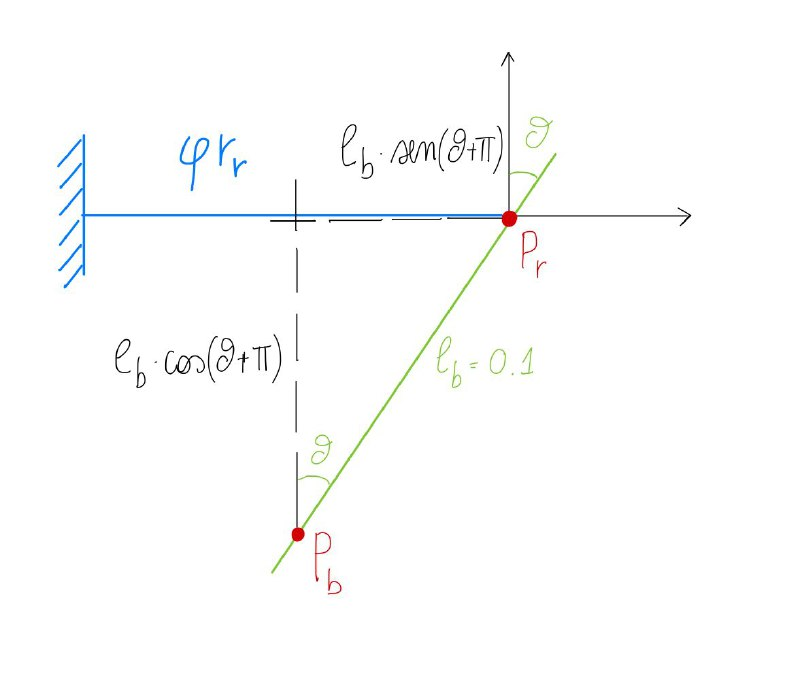
\includegraphics[width=0.6\textwidth]{Immagini/ChassisAngle.jpg}
 		\caption{Ragionamento per il calcolo dei contributi dinamici dello chassis}
 		\label{fig:chassis}
 	\end{figure}
 	
\end{itemize}

\chapter{Equazioni del moto}
Una volta definita la dinamica del sistema ed ottenuta quindi l'equazione di Lagrange che ne caratterizza il comportamento, andiamo a ricavare le equazioni del moto, le quali consentono di definire l'andamento delle \textit{coordinate libere} (scelte in fase inziale di progetto) che sappiamo essere
\begin{itemize}
	\item $\phi = q_1 =$ \textit{angolo di rotazione delle ruote}
	\item $\theta = q_2 =$ \textit{angolo di inclinazione dello chassis}
\end{itemize}

In particolare possiamo definire le cosidette \textit{equazioni di Eulero-Lagrange}, ovvero un insieme di n equazioni differenziali (con n pari al numero di coordinate libere del sistema), la cui risoluzione fornisce le equazioni del moto del sistema.
\begin{center}
	\label{eq:lagrangiana}
	$\frac{d}{\mathrm{dt}}\left(\frac{\partial }{\partial \dot{q} }L\right)-\frac{\partial }{\partial q}L=\mathrm{torque}\ $
\end{center}

Sono da effettuare alcune annotazioni sugli addenti presenti nell'equazione ~\ref{eq:lagrangiana}:
\begin{itemize}
	\item \textit{q} rappresenta la coordinata libera (nel nostro caso sarà $\theta$ e $\phi$);
	\item al secondo membro della lagrangiana TODO
	\item molto importante ai fini della correttezza delle equazioni  del moto è il valore da assegnare a \textit{torque}; infatti esso varia a seconda che il sistema agisca sulla coordinata libera \textit{q} a valle o a monte della trasmissione.
	Nello specifico, si osserva che il motore è composto da due parti: lo statore e il rotore. Esse trasmettono una coppia uguale e inversa a ciò cui sono collegati: lo statore, posizionato nella base del Segway, influenza la coordinata $\theta$ ed esercita una coppia sullo chassy pari ad una generica \textit{$-2 C_m$}; il fattore moltiplicativo 2 è dovuto al fatto che nella base sono presenti due motori.
	Parimenti, il rotore trasmette all'albero motore una coppia \textit{$C_m$}. A valle della trasmissione si misura dunque una coppia \textit{$\frac{C_m}{\tau}$} dovuta alla presenza della trasmissione; questa coppia ridotta all'albero dell'utilizzatore è la coppia che in definitiva va ad agire sulle ruote e quindi sulla coordinata $\phi$
\end{itemize}
Si ottiene dunque il seguente sistema di equazioni:
\begin{center}
	\label{eq:lagrangiana_theta_phy}
	$\frac{d}{\mathrm{dt}}\left(\frac{\partial }{\partial \dot{\theta} }L\right)-\frac{\partial }{\partial \theta}L=\mathrm{-2 C_m}\ $\\
	$\frac{d}{\mathrm{dt}}\left(\frac{\partial }{\partial \dot{\phi} }L\right)-\frac{\partial }{\partial \phi}L=\mathrm{\frac{C_m}{\tau}}\ $
\end{center}
dove $\tau$ è il rapporto di trasmissione calcolato come segue:
\begin{center}
	\label{eq:tau}
	$\tau_1 = 0.1$\\
	$\tau_2 = \frac{Z_in}{Z_out} = \frac{22}{26}$\\
	$\tau = \tau_1 \cdot{\tau_2} = 0.085$	
\end{center}

La risoluzione delle equazioni \ref{eq:lagrangiana_theta_phy}, permette di ottenere due equazioni differenziali del secondo ordine che il comando \textit{matlabFunction()} va a scrivere in una funzione di matlab: questa funzione avrà come input i valori da cui dipendono le equazioni differenziali e moltiplicandoli tra di loro da come output il valore di $\ddot{\theta}$ e $\ddot{\phi}$.
TODO (mettere le dipendende di theta pp e phi pp)

\subsection{Linearizzazione} TODO linearizzazione attorno alla massa 70 kg
Il passo successivo che è stato svolto riguarda la linearizzazione; linearizzare è importante poiché il controllore viene progettato sul sistema lineare e poi testato sul sistema reale e quindi non lineare.

Per tale ragione è necessario innanzitutto calcolare l'equilibrio del sistema, cioè il punto in cui $\ddot{\theta} = 0$:
\begin{center}
	$$\left(\begin{array}{c}
		-0.01174364-\text{7.105427e-15}\,\mathrm{i}\\
		3.129849-\text{7.105427e-15}\,\mathrm{i}
	\end{array}\right)$$
\end{center}

I risultati ottenuti sono, circa, numeri naturali e rispondono a quanto ci aspettavamo: 
\begin{itemize}
	\item il sistema ha due equilibri, il primo $\theta = -0.01174364$ ci si aspetta che sia instabile in quanto il baricentro del sistema V.A.B. più Uomo è sopra all'asse delle ruote
	\item  $\theta = 3.129849$ è un equilibrio stabile poiché il baricentro sta sotto l'asse delle ruote e un eventuale disturbo, dopo un transitorio, risulterebbe avere effetto nullo sul sistema.
\end{itemize}

Ovviamente, ai fini del controllo, si è linearizzato attorno al primo equilibrio; non avrebbe senso cpntrollare il sistema quando questo risulta capovolto.
Il vettore degli stati e delle uscite sono i seguenti:
\begin{center}
	$$
	x=\left\lbrack \begin{array}{c}
		x_1 \to \phi \;\\
		x_2 \to \dot{\phi \;} \\
		x_{3\;} \to \theta \;\\
		x_4 \to \dot{\theta \;} 
	
		\end{array}\right\rbrack
	$$
	
	$$
	y=\left\lbrack \begin{array}{c}
	y_1\;\\
	y_2\;
	
\end{array}\right\rbrack
	$$
\end{center}
e vengono definite anche alcune variabili di supporto:
\begin{center}
	$$
	\overset{\bullet \;}{x_1 \left(t\right)} =\bar{x_2 } =0\to f_1
	$$
	$$
	\overset{\bullet \;}{x_2 \left(t\right)} =\overset{\bullet \bullet \;\;}{\phi \;} \to f_2
	$$
	$$
	\overset{\bullet \;}{x_3 \left(t\right)} =\bar{x_4 } =0\to f_{3\;}
	$$
	$$
	\overset{\bullet \;}{x_4 \left(t\right)=} \overset{\bullet \bullet \;\;}{\theta \;} \to f_4
	$$
	$$
	y_{1\;} \left(t\right)=\phi =x_{1\;} \to g_1
	$$
	$$
	y_{2\;} \left(t\right)=\theta =x_{2\;} \to g_2
	$$
\end{center}

ricordando che un generico sistema dinamico può essere scritto come:
\begin{center}
	$$
	G\left(s\right)=C\bullet {\left(\mathrm{sI}-A\right)}^{-1} \bullet B+D
	$$
\end{center}
allora:
\begin{center}
	$$
	A=\left\lbrack \begin{array}{cccc}
	\frac{\partial }{\partial x_1 }f_{1\;}  & \frac{\partial }{\partial x_2 }f_{1\;}  & \frac{\partial }{\partial x_3 }f_{1\;}  & \frac{\partial }{\partial x_4 }f_{1\;} \\
	\frac{\partial }{\partial x_1 }f_{2\;}  & \frac{\partial }{\partial x_2 }f_{2\;}  & \frac{\partial }{\partial x_3 }f_{2\;}  & \frac{\partial }{\partial x_4 }f_{2\;} \\
	\frac{\partial }{\partial x_1 }f_3  & \frac{\partial }{\partial x_2 }f_3  & \frac{\partial }{\partial x_3 }f_3  & \frac{\partial }{\partial x_4 }f_3 \\
	\frac{\partial }{\partial x_1 }f_4  & \frac{\partial }{\partial x_2 }f_4  & \frac{\partial }{\partial x_3 }f_4  & \frac{\partial }{\partial x_4 }f_4 
	\end{array}\right\rbrack
	$$
	$$
	B=\left\lbrack \begin{array}{c}
	\frac{\partial }{\partial u}f_1 \\
	\frac{\partial }{\partial u}f_2 \\
	\frac{\partial }{\partial u}f_3 \\
	\frac{\partial }{\partial u}f_4 
	\end{array}\right\rbrack
	$$
	$$
	C=\left\lbrack \begin{array}{cccc}
	\frac{\partial }{\partial x_1 }g_{1\;}  & \frac{\partial }{\partial x_2 }g_{1\;}  & \frac{\partial }{\partial x_3 }g_{1\;}  & \frac{\partial }{\partial x_4 }g_{1\;} \\
	\frac{\partial }{\partial x_1 }g_{1\;}  & \frac{\partial }{\partial x_2 }g_{1\;}  & \frac{\partial }{\partial x_3 }g_{1\;}  & \frac{\partial }{\partial x_4 }g_2 
	\end{array}\right\rbrack
	$$
	$$
	\;D=\left\lbrack \begin{array}{cc}
	\frac{\partial }{\partial u}g_{1\;}  & \frac{\partial }{\partial u}g_2 
	\end{array}\right\rbrack
	$$
\end{center}

Sostituendo i valori numerici dei vari simboli si ottengono le seguenti matrici:

\begin{center}
		$$
		\left(\begin{array}{c}
		\frac{2.75}{s^2 }-\frac{\text{1.749e+13}}{\text{2.392e+13}\,s^2 -\text{4.398e+12}\,s^4 }\\ \\
		\frac{2.75}{s}-\frac{\text{1.749e+13}}{\text{2.392e+13}\,s-\text{4.398e+12}\,s^3 }\\ \\
		-\frac{\text{1.149e+12}}{\text{4.398e+12}\,s^2 -\text{2.392e+13}}\\ \\
		-\frac{\text{1.149e+12}\,s}{\text{4.398e+12}\,s^2 -\text{2.392e+13}}
		\end{array}\right)
		$$
\end{center}
Si può notare come la prima e la seconda riga della matrice differiscano solo per un fattore derivativo, così come la terza e quarta riga; questo è ovvio ed atteso in quanto $x_2$ è a derivata di $x_1$ e $x_4$ la derivata di $x_3$
